\documentclass[12pt]{aghdpl}
% \documentclass[language=en,11pt]{aghdpl}  % praca w języku angielskim

%---------------------------------------------------------------------------

\usepackage{listings}

% Abstrakt
\newenvironment{abstractpage}
{\cleardoublepage\vspace*{\fill}\thispagestyle{empty}}
{\vfill\cleardoublepage}
\renewenvironment{abstract}[1]
{\bigskip\selectlanguage{#1}%
    \begin{center}\bfseries\abstractname\end{center}}
{\par\bigskip}


\author{Michał Machura}
\shortauthor{M. Machura}

%\titlePL{Przygotowanie bardzo długiej i pasjonującej pracy dyplomowej w~systemie~\LaTeX}
%\titleEN{Preparation of a very long and fascinating bachelor or master thesis in \LaTeX}

\titlePL{Detekcja obiektów z wykorzystaniem głębokich sieci neuronowych zrealizowana na wbudowanej platformie obliczeniowej}
\titleEN{Object detection using deep neural networks implemented on an embedded computing platform}


\shorttitlePL{Detekcja z wykorzystaniem DNN zrealizowana na wbudowanej platformie obliczeniowej} % skrócona wersja tytułu jeśli jest bardzo długi
% \shorttitleEN{Detection using DNN implemted on an embeded computing platform}


% Dopuszczalne wartości[1,2]:
% * "Projekt dyplomowy" - na koniec studiów I stopnia
% * "Praca dyplomowa" - na koniec studiów II stopnia
% [1] Zasady dyplomowania w roku akademickim 2020/2021 (Decyzja Dziekana WEAIiIB nr 16/2020 z dnia 9 grudnia 2020 roku)
% [2] Załącznik nr 1a) do Decyzji nr 16/2020 Dziekana Wydziału EAIiIB z dnia 09 grudnia 2020 r.

\thesistype{Praca dyplomowa}
%\thesistype{Master of Science Thesis}

\supervisor{dr inż. Tomasz Kryjak}

\degreeprogramme{Automatyka i Robotyka}
%\degreeprogramme{Automatics and Robotics}

\date{2021}

%\department{Katedra Informatyki Stosowanej}
%\department{Department of Applied Computer Science}

\faculty{Wydział Elektrotechniki, Automatyki, Informatyki i Inżynierii Biomedycznej}
%\faculty{Faculty of Electrical Engineering, Automatics, Computer Science and Biomedical Engineering}

% \acknowledgements{Serdecznie dziękuję }


\begin{document}

	\titlepages
	
	\begin{abstractpage}
    \begin{abstract}{polish}
        W ramach niniejszej pracy zaimplementowano aplikację do automatycznej rejestracji przebiegu gry w~brydża sportowego. Została ona wykonana w oparciu o system wizyjny, przetwarzający obraz nagrany przez układ dwóch kamer skierowanych na stół, przy którym rozgrywane jest rozdanie brydżowe. 
        Pierwszym etapem realizacji zadania jest właściwa detekcja i klasyfikacja elementów wykorzystywanych podczas gry -- kart oraz zapowiedzi licytacyjnych. W tym celu wykorzystano dwie głębokie konwolucyjne sieci neuronowe YOLOv4. Podczas procesu uczenia, który został zrealizowany z wykorzystaniem automatycznie wygenerowanej bazy zdjęć, uzyskano detektor charakteryzujący się ponad 99.9\% skutecznością na zbiorze testowym. Druga część systemu odpowiedzialna jest za analizę uzyskanych informacji i w oparciu o zasady gry odtworzenie jej przebiegu.
        Przygotowana aplikacja została przetestowana na zebranym podczas zawodów brydżowych materiale wideo i charakteryzuje się wysoką skutecznością. Drobne modyfikacje oraz akceleracja sprzętowa mogłyby umożliwić wykorzystanie systemu do przygotowania transmisji na żywo z zawodów brydżowych. 
       
        \bigskip
        \textbf{Słowa kluczowe:}   głębokie konwolucyjne sieci neuronowe, system wizyjny, detekcja obiektów, brydż sportowy
       
       
    \end{abstract}
    \bigskip
    \bigskip
    \bigskip
    \bigskip
    \bigskip
    \bigskip
    \bigskip
    \bigskip
    \bigskip
    \bigskip
    \bigskip
    \begin{abstract}{english}
        In this work, the implementation of an application for automatic registration of a duplicate bridge game is presented. It is based on a vision system that processes images recorded by a system of two cameras directed at the table where the game takes place.
        The first stage of the task is the detection of elements used during play -- cards and bidding calls. For this purpose, two YOLOv4 deep convolutional neural networks were used. During the training process, which was carried out using an automatically generated dataset, we obtained a detector characterised by more than 99.9\% accuracy on the test set. The second part of the system is responsible for analysing the obtained information and, based on the rules of the game, reconstructing its course.
        The prepared application has been tested on video collected during bridge competitions and is characterised by its high accuracy. Minor modifications and hardware acceleration could make it possible to use the system for preparing live broadcasts of bridge competitions. 
        
        \bigskip
       
        \textbf{Keywords:} Deep Convolutional Neural Networks, vision system, object detection, dupliacte bridge
    \end{abstract}
\end{abstractpage}


	\RedefinePlainStyle
	
	\setcounter{tocdepth}{2}
	\tableofcontents
	\clearpage
	
	\newcommand{\round}[1]{\ensuremath{\lfloor#1\rceil}}
	
	\chapter{Wprowadzenie}
\label{cha:wprowadzenie}

Rozwój technologi takich jak pojazdy autonomiczne, roboty humanoidalne, systemy nadzorcze czy systemy automatycznej kontroli wymagają stosowania rozwiązań o wysokiej skuteczności.
We wspomnianych technologiach, często wymagane jest rozpoznawania otoczenia w czasie rzeczywistym.
Możliwe jest to miedzy innymi poprzez realizację zadania detekcji wybranych typów obiektów za pomocą systemów percepcji takich jak \emph{LiDAR} czy kamery. 

Rozwiązaniami cechującymi się wysoką skutecznością są algorytmy sztucznej inteligencji, a w szczególności sieci neuronowe.
Rozwiązania te jednak cechują się wysoką złożonością obliczeniową.
W przypadku systemów stacjonarnych problem ten można rozwiązać poprzez zastosowanie urządzeń zapewniających dużą moc obliczeniową takich jak karty graficzne.
Rozwiązanie to jednak nie zawsze jest możliwe dla zastosowań mobilnych wymagających technologii o niskim zużyciu energii.
W takich sytuacjach korzystnym wydaje się być zastosowanie układów \emph{FPGA}
oraz tzw. sieci kwantyzowanych (ang. \emph{Quantized Neural Networks}).
Rozwiązania te pozwalają osiągać zarówno wysoką skuteczność, niewielkie zużycie energii jak i wysoką przepustowość pozwalającą na zastosowanie w systemach czasu rzeczywistego.

\section{Cele pracy}
\label{sec:celePracy}
Celem niniejszej pracy jest implementacja głębokiej sieci neuronowej na wbudowanej platformie obliczeniowej - układzie \emph{Zynq UltraScale+ MPSoC}.
System jest opracowywany na potrzeby konkursu \emph{2021 DAC SDC}.
Zadaniem jest detekcja obiektów na zdjęciach zarejestrowanych przez drona. 
Wymagane jest osiągnięcie wysokiej przepustowości oraz skuteczności, przy jednoczesnym niewielkim zużyciu energii. 
Do tego celu należy przeprowadzić niezbędne badania literatury pozwalające na zaproponowanie własnego rozwiązania problemu wykorzystującego akcelerację sprzętową obliczeń.

%---------------------------------------------------------------------------

\section{Zawartość pracy}
\label{sec:zawartoscPracy}
W pracy przedstawiono zagadnienia związane z uczeniem sieci neuronowych, a także ich implementacją. Ze względu na uczestnictwo w konkursie w rozdziale \ref{cha:Analiza probemu} przedstawiono szczegółowe wymagania i założenia dotyczące m.in. implementacji i oceny rozwiązania. Przedstawiono także opis docelowej platformy obliczeniowej oraz omówiono narzędzia wspomagające implementacje sprzętową.
W rozdziale \ref{ch:detekcja} zrealizowano przegląd metod detekcji klasycznych oraz opartych o sieci neuronowe, w szczególności o rozwiązania energooszczędne.
Badania nad architekturą oraz proces uczenia i kwantyzacji zostały opisane w rozdziale \ref{cha:Badania wstępne}.
Rozdział \ref{cha:Implementacja} przedstawia implementację opracowanej architektury zarówno programową jak i sprzętową. 
Uzyskane rezultaty oraz przeprowadzoną optymalizację zawarto w rozdziale \ref{cha:Optymalizacja}. 
W rozdziale \ref{cha:Podsumowanie} podsumowano pracę oraz przedstawiono wnioski z niej płynące. 


	\chapter{Analiza problemu}
\label{cha:Analiza probemu}
(Co do tej nazwy rozdziału to mam wątpliwości, 
ale na ten czas nic lepszego nie wymyśliłem,
-zapewne do zmiany)

\section{Wymagania}
- wymagania konkursu
- wymagane pliki,
- platforma(i jej opis) itp.

\section{Przegląd rozwiązań}
- analiza sieci YOLO z ultranet, SkyNet
- QNN i BNN
- (ten pod rozdział można by potraktować poniekąd jako przegląd literatury o sieciach/rozwiązaniach energooszczędnych)

\section{Narzędzia}
Przegląd narzędzi wspomagających implementację sprzętową:
- Vitis AI
- FINN + Brevitas
- QKeras
- DNN Builder



%---------------------------------------------------------------------------

    


	\chapter{Badania wstępne}
\label{cha:Badania wstępne}

Analiza rozpatrywanego problemu detekcji wraz ze sprzętową implementacją pozwala na zaproponowanie możliwych rozwiązań. W niniejszym rozdziale zostaną przedstawione propozycje architektur sieci, proces ich uczenia a także kwantyzacji. 

\section{Architektura wstępna} %section{Architektura wstępna}

%}
% Liczba parametrów sieci \emph{Ultra\_net} wynosi ponad 200 tys..
Liczba parametrów sieci \emph{SkyNet}\footnote{W wersji bez połączenia typu \emph{bypass}} wynosi ponad $300$ tys. 
Zastosowanie separowalnych konwolucji skutkuje znaczną redukcją liczby parametrów względem architektury wykorzystującej pełną konwolucję - powyżej $2.6$ miliona parametrów \footnote{Architektur tych nie można w pełni ze sobą utożsamiać jako substytutów.}. 
Tak znaczna redukcja (również złożoności obliczeniowej) skłania do zastosowania konwolucji separowalnych dla sprzętowej akceleracji. 
W tym celu rozważono architekturę sieci o 9 warstwach konwolucji separowalnej (z bias) z funkcją aktywacji $ReLU$ po konwolucji typu pointwise. Architektura posiada również warstwy Max Pooling po każdej konwolucji separowalnej.
Ostatnia warstwa stanowi warstwę podobną do warstwy \emph{YOLOv1}. Na rysunku \ref{fig:arch_v1} przedstawiono graficzną reprezentację architektury. 
Jako wejście sieci pozostawiono oryginalne wymiary obrazów dostępnych w zbiorze treningowym.

Ze względu, iż rozpatrywany problem to detekcja bez klasyfikacji, pominięto w funkcji błędu \eqref{eq:lossv1} część związaną z klasyfikacją. 
Jako wartości referencyjne dla wyjść sieci wykorzystano maskę $y_{ref}$ (o wymiarach 5x7x12) z odpowiadającymi wartościami dla kanałów. Równania \eqref{eq:y_ref_valv1}-\eqref{eq:y_ref_hv1} prezentują sposób wyznaczenia wartości referencyjnych dla elementów poszczególnych kanałów. 

\begin{figure}
    \centering
    \includegraphics[width=\linewidth]{images/arch_v1.png}
    \caption{Wstępna architektura sieci dla zadania detekcji, wykorzystująca konwolucje separowalne oraz warstwę podobną do \emph{YOLOv1}. Architektura posiada niespełna 43 tys. parametrów.}
    \label{fig:arch_v1}
\end{figure}

\begin{equation}
y_{ref}_{0,i,j} = 
\begin{cases}
    1, & \text{if }  i = row \And j = col \\
    0,              & \text{otherwise}
\end{cases}
\label{eq:y_ref_valv1}
\end{equation}

\begin{equation}
y_{ref}_{1,i,j} = 
\begin{cases}
    x_c \frac{12}{640} - col - 0.5, & \text{if }  i = row \And j = col \\
    0,              & \text{otherwise}
\end{cases}
\label{eq:y_ref_xv1}
\end{equation}

\begin{equation}
y_{ref}_{2,i,j} = 
\begin{cases}
    y_c \frac{7}{360} - row - 0.5, & \text{if }  i = row \And j = col \\
    0,              & \text{otherwise}
\end{cases}
\label{eq:y_ref_yv1}
\end{equation}

\begin{equation}
y_{ref}_{3,i,j} = 
\begin{cases}
    log(\frac{w}{a_w}) & \text{if }  i = row \And j = col \\
    0,              & \text{otherwise}
\end{cases}
\label{eq:y_ref_wv1}
\end{equation}

\begin{equation}
y_{ref}_{4,i,j} = 
\begin{cases}
    log(\frac{h}{a_h}) & \text{if }  i = row \And j = col \\
    0,              & \text{otherwise}
\end{cases}
\label{eq:y_ref_hv1}
\end{equation}

$row$ oraz $col$ oznaczają indeks siatki wyjściowej do którego został przypisany referencyjny obiekt, $a_w$ oraz $a_h$ odpowiednio szerokość i wysokość \emph{anchor box}. 
Przyjęto  $a_w = 16$ oraz $a_h = 16$ jako wartość łączna wartość kroku sieci (ang. \emph{stride}) wynikająca z liczby warstw Max Pooling.
Przyjmując za $x_c, y_c, w, h$ odpowiednio współrzędne położenia środka obiektu oraz jego wymiary, można wyznaczyć indeksy $row$ oraz $col$ według wzorów \eqref{eq:rowv1}-\eqref{eq:colv1}.

\begin{equation}
col = \round{x_c \frac{12}{640} - 0.5}
\label{eq:colv1}
\end{equation}
\begin{equation}
row = \round{y_c \frac{7}{360} - 0.5}
\label{eq:rowv1}
\end{equation}


Błąd wykrycia obiektu został zdefiniowany jako entropia binarna $BCE$. 
Błąd przesunięcia od centrum siatki detekcji (wynikającej z wymiarów ostatniej warstwy) został zdefiniowany jako średni błąd bezwzględny $MAE$. Błąd wymiarów został zdefiniowany jako wartość średnia pierwiastka $MSQRT$ z wartości bezwzględnej różnicy pomiędzy odpowiedzią sieci oraz wartością referencyjną.
Funkcję błędu (reprezentowaną przez równanie \eqref{eq:lossv1}) dla całej sieci stanowi ważona suma błędów składowych ze współczynnikami $\lambda_obj, \lambda_xy oraz \lambda_wh$. 

\begin{equation}
\begin{aligned}
loss =& \lambda_{obj} BCE(\sigma(y_{pred}_{0,:,:}), y_{ref}_{0,:,:}) \\
&+ \frac{\lambda_{xy}}{2}( MAE(y_{pred}_{1,:,:}, y_{ref}_{1,:,:}) + MAE(y_{pred}_{2,:,:}, y_{ref}_{2,:,:})) \\
&+ \frac{\lambda_{wh}}{2} (MSQRT(|y_{pred}_{3,:,:} - y_{ref}_{3,:,:}|) + MSQRT(|y_{pred}_{4,:,:} - y_{ref}_{4,:,:}|))
\end{aligned}
\label{eq:lossv1}
\end{equation}


Przed rozpoczęciem procesu uczenia dokonano podziału dostępnego zbioru uczącego na trzy zbiory: uczący, walidacyjny oraz testowy w stosunku 81:9:10. Podział został przeprowadzony losowo wewnątrz każdej sekwencji.
Uzyskany podział zbioru był stosowany dla wszystkich dalszych wariantów architektur i funkcji błędu.

Rozpoczynając trening sieci ustalono wszystkie parametry funkcji błędu \eqref{eq:lossv1} na wartość $1$.
Dla zbioru uczącego przeprowadzano augmentację danych\footnote{Dla pozostałych wariantów architektur również przeprowadzano augmentację danych.} z wykorzystaniem filtracji uśredniającej, zakłóceń addytywnych, przeskalowania czy też rotacji.
Do minimalizacji błędu użyto algorytmu \emph{Adadelta}\footnote{Dla pozostałych architektur również użyto tego algorytmu.}.

Proces uczenia przerwano, gdy nie zauważono zmian wartości błędu oraz metryki IoU dla zbioru uczącego oraz walidacyjnego.
Finalnie architektura osiągnęła wartość współczynnika $iou = 0.47$ dla zbioru walidacyjnnego.

\section{Architektura rozgałęziona}
Ze względu na niewielką wartość współczynnika $iou$, architekturę zmodyfikowano o dodanie dodatkowego wyjścia z sieci pochodzącego z warstwy pośredniej zakończonego warstwą analogicznie do wersji nierozgałęzionej (wymiary \emph{anchor box} dla rozgałęzienia $a_w = 8$ oraz  $a_h = 8$). Na rysunku \ref{fig:arch_v2} przedstawiono graficzną reprezentację architektury. Po przeprowadzeniu procesu ucznia sieci, z wykorzystaniem techniki transferu wiedzy z architektury pierwotnej, uzyskano pogorszenie wartości $iou$. 

\begin{figure}
    \centering
    \includegraphics[width=\linewidth]{images/Architektura_branched.png}
    \caption{Architektura rozgałęziona wykorzystująca konwolucje separowalne.}
    \label{fig:arch_v2}
\end{figure}


\section{Architektura Resnet18}
Rezultaty dotychczas badanych architektur były niewystarczające. Rozważono wówczas architekturę wykorzystującą połączenia residualne - \emph{Resnet18}\cite{resnet18}. 
W tym celu wykorzystano dwa pierwsze bloki residualne (sieci przetrenowanej na zbiorze danych \emph{ImageNet}\cite{imagenet} dostępnej za pośrednictwem biblioteki \emph{PyTorch}) oraz dodano warstwę \emph{Yolov2}\cite{yolov2} poprzedzoną warstwą konwolucyjną ze 128 filtrami. 
Wykorzystano tu trzy \emph{anchor box} o wymiarach(szerokość x wysokość): $22x33, 43x69, 89x133$ uzyskanych jako wynik algorytmu k-średnich. 
Uzyskana architektura podsiadała ponad 700 tys. paramterów.
Wymiary obrazów wejściowych zredukowano do 360 pikseli szerokości oraz 180 pikseli wysokości.
Funkcja błędu odpowiedzi sieci przyjmuje postać daną równaniem \eqref{eq:loss_yolo_v2}.
Jako funkcję błędu regresji $loss_{bbox}$ wybrano funkcję \emph{GIoU}\cite{giou}. Dla błędu wykrycia obiektu zastosowano (podobnie jak dla poprzednich architektur) entropię binarną. Dla obu współczynników wagowych przyjęto wartość $1$.
\begin{equation}
loss = \lambda_{validity} BCE(y_{pred}_{0:2,:,:}, y_{ref}_{0:2,:,:}) + \lambda_{bbox} loss_{bbox}(y_{pred}_{3:14,:,:}, x_c,y_c,w,h)
\label{eq:loss_yolo_v2}
\end{equation}


Dla modelu zmiennoprzecinkowego architektura osiągnęła wartość $iou$ ponad $0.8$ dla zbioru walidacyjnego. Proces uczenia został przerwany podobnie jak poprzednio, gdy nie zauważano znacznych zmian błędu i metryki \emph{IoU}.

Zdecydowano się na kwantyzację modelu z wykorzystaniem zapisu stałoprzecinkowego. 
Obraz wejściowy został poddany kwantyzacji 8 bitowej bez znaku i bez części całkowitej. 
Wagi oraz wyjścia warstw pośrednich poddano kwantyzacji 8 bitowej ze znakiem i 2 bitami części całkowitej.
Ostanie dwie warstwy poddano kwantyzacji 8 bitowej ze znakiem i 3 bitami części całkowitej.
W przypadku każdej kwantyzacji zastosowano również ograniczenie wartości wynikowej do limitów wynikających z zapisu w formacie stałoprzecinkowym.

Następnie po zakończeniu treningu sieci z kwantyzacją osiągnięto wartość $iou = 0.72$.
Uzyskana wartość pozwalałaby na osiągnięcie maksymalnej wartości oceny\footnote{Jeżeli uzyskano by podobny rezultat na zbiorze tajnym.} danej równaniem \eqref{eq:iou_score}. 

Rozważana architektura wydaje się być trudniejsza do sprzętowej implementacji ze względu na połączenia residualne oraz znaczne rozmiary. 
Jednakże analizując przeprowadzone procesy uczenia można zauważyć, iż dodanie warstw normalizujących oraz zastosowanie funkcji błędu bazującej na metryce \emph{IoU} pozwala na osiągnięcie większych wartości \emph{IoU}, przy mniejszej liczbie epok treningowych \footnote{Dla poprzednich architektur liczba epok była znacznie większa, niż dla architektury residualnej}. 


\section{LittleNet}

Podsumowując wnioski z rozważanych dotychczas architektur można stwierdzić, iż:
\begin{itemize}
    \item zastosowanie konwolucji separowalnych pozwala na znaczną redukcję liczby parametrów oraz złożoności obliczeniowej, 
    \item warstwy normalizacji pozwalają zmniejszyć liczbę epok treningowych,
    \item funkcja błędu bazująca na matryce \emph{IoU} pozwala osiągnąć lepsze wyniki.
\end{itemize}

Dodatkowo można zauważyć, konwolucja separowalna dla pierwszej warstwy posiada jedynie trzy filtry typu depthwise.
Następna warstwa typu pointwise dokonuje podziału w przestrzeni zaledwie trójwymiarowej. 
Może to skutkować pewną utratą znacznej części informacji już na początkowym etapie przetwarzania, a także pewną redundancją filtrów pointwise lub ich wrażliwości na nie wielkie zmiany wejścia. 
Zastosowanie pełnej konwolucji w pierwszej warstwie mogłoby polepszyć jakość detekcji.
Jednakże kownolucje pełne są bardziej złożone w implementacji sprzętowej. 
Z tego względu zdecydowano się na zastosowanie wielokrotnej filtracji typu depthwise. 
Pozwala to na zwiększenie liczby cech bezpośrednio ekstrahowanych z obrazu wraz z zachowaniem możliwości stosunkowo łatwej implementacji sprzętowej.

Proponowaną architekturę przedstawiono na rysunku \ref{fig:LN_arch}. 
Sieć zawiera 7 bloków z konwolucją typu depthwise oraz 7 z konwolucją typu pointwise. Po każdej konwolucji występuje warstwa normalizacyjna oraz funkcja aktywacji $ReLU$. Pierwszy blok zawiera warstwę depthwise posiada z 5 filtrami na kanał, kolejne bloki zawierają już tylko po 2 filtry na kanał.
Po pierwszych 4 warstwach pointwise  występuje warstwa Max Pooling. 
Ostatnią warstwę stanowi konwolucja typu pointwise stanowiąca warstwę \emph{YOLOv2}. Wymiary \emph{anchor box} pozostały takie same jak dla architektury wykorzystującej bloki residualne, lecz przeskalowane do wymiarów wejścia sieci. 
Proponowana architektura posiada niespełna 134 tys. parametrów, co stanowi znaczą redukcję liczby parametrów w stosunku do \emph{SkyNet} (powyżej 300 tys.) oraz \emph{Ultra\_net} (ponad 200 tys.). 
Architekturze nadano % roboczą
nazwę \emph{LittleNet}.
\begin{figure}
    \centering
    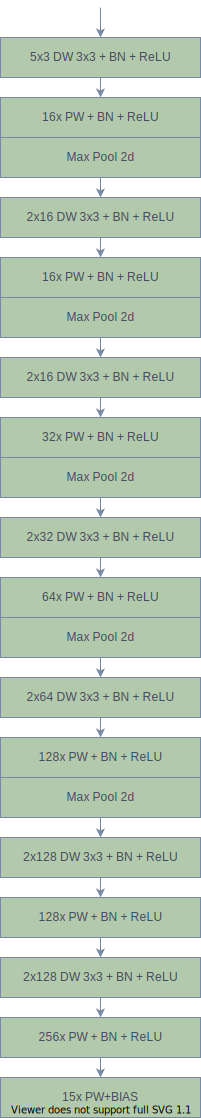
\includegraphics[width=4cm]{images/LNv1}
    \caption{Proponowana architektura sieci \emph{LittleNet}.}
    \label{fig:LN_arch}
\end{figure}

Rozmiar wejścia sieci ustalono na 360 pikseli szerokości oraz 180 pikseli wysokości.
Funkcja błędu odpowiedzi sieci \eqref{eq:loss_yolo_v2} rozszerzono o regularyzację normą $L_1$ parametrów sieci $p$, uzyskując równanie \eqref{eq:loss_yolo_v2_reg}. .
\begin{equation}
\begin{aligned}
loss =& \lambda_{validity} BCE(y_{pred}_{0:2,:,:}, y_{ref}_{0:2,:,:}) \\
&+ \lambda_{bbox} loss_{bbox}(y_{pred}_{3:14,:,:}, x_c,y_c,w,h)\\
&+ \lambda_{reg} L_1(p)
\end{aligned}
\label{eq:loss_yolo_v2_reg}
\end{equation}
Za funkcję błędu regresji $loss_{bbox}$  przyjęto funkcję \emph{GCIoU} daną równaniem \eqref{eq:gciou}. 
Funkcja ta bazuje na \emph{GIoU}\cite{giou}, \emph{DIoU}\cite{dciou} oraz \emph{CIoU}\cite{dciou}. 
Połączenie powyższych funkcji pozwala na połączenie ich zalet funkcji: 
\begin{itemize}
    \item \emph{GIoU} - bardziej bezpośredni wpływ błędu na parametry (gdy \emph{IoU}$ = 0$),
    \item \emph{DIoU} - centralizacji predykcji,
    \item \emph{CIoU} - wzmocnione finalne skalowanie rozmiaru. 
\end{itemize}
\begin{equation}
GCIoU = GIoU + CIoU + IoU - 1
\label{eq:gciou}
\end{equation}
Ustalono parametry wagowe na $\lambda_{validity} = 20$, $\lambda_{bbox} = 1$ oraz $\lambda_{reg} = 0.01$.
Krok uczący został początkowo ustalony jako $l_r=1$. 
W trakcie procesu uczenia podlegał on modyfikacją zgodnie z równaniami \eqref{eq:lr_1} oraz \eqref{eq:lr_2}.
\begin{equation}
l_r_(t+1) = 
\begin{cases}
    1.3*l_r(t), &\text{if } loss(t) < loss(t-1) \\
    0.5*l_r(t), &\text{if } loss(t) > loss(t-1) \\
    l_r(t), &\text{otherwise}
\end{cases}
\label{eq:lr_1}
\end{equation}
\begin{equation}
l_r(t+1) = max(10^{-5}, min(1, l_r(t+1)))
\label{eq:lr_2}
\end{equation}


Po zakończeniu procesu uczenia modelu zmiennoprzecinkowego osiągnięto wartość $iou = 0.8$ dla zbioru walidacyjnego oraz $0.7$ dla zbioru uczącego. 
Powodem tak znacznej różnicy wartości metryki jest znaczny stopień augmentacji danych.

Sieć poddano kwantyzacji. Dane wejściowe zostały poddane kwantyzacji 8 bitowej bez znaku i bez części całkowitej.
Warstwy pośrednie poddano kwantyzacji 8 bitowej ze znakiem i 2 bitami części całkowitej.
Ostatnią warstwę poddano kwantyzacji 8 bitowej ze znakiem i 3 bitami części całkowitej.

Uzyskano wartość $iou = 0.76$ dla zbioru walidacyjnego oraz $0.67$ dla zbioru uczącego.
Na rysunkach \ref{fig:float_loss}-\ref{fig:quant_iou} przedstawiono przebiegi funkcji błędu oraz metryki \emph{IoU} dla modelu zmiennoprzecinkowego oraz kwantyzowanego.

\begin{figure}
     \centering
     \begin{subfigure}[b]{0.49\textwidth}
         \centering
         \includegraphics[width=\textwidth]{images/float32_hist_of_loss.png}
         \caption{}
         \label{fig:float_loss}
     \end{subfigure}
     \hfill
     \begin{subfigure}[b]{0.49\textwidth}
         \centering
         \includegraphics[width=\textwidth]{images/float32_hist_of_iou.png}
         \caption{}
         \label{fig:float_iou}
     \end{subfigure}
     \hfill
     \begin{subfigure}[b]{0.49\textwidth}
         \centering
         \includegraphics[width=\textwidth]{images/8_bit_quant_hist_of_loss.png}
         \caption{}
         \label{fig:quant_loss}
     \end{subfigure}
     \hfill
     \begin{subfigure}[b]{0.49\textwidth}
         \centering
         \includegraphics[width=\textwidth]{images/8_bit_quant_hist_of_iou.png}
         \caption{}
         \label{fig:quant_iou}
     \end{subfigure}
     \hfill
     
    \caption{Przebiegi wartości błędu oraz metryki \emph{IoU} (w zależności od epoki uczącej) dla modelu zmiennoprzecinkowego \ref{fig:float_loss} i \ref{fig:float_iou} oraz \ref{fig:quant_loss} i \ref{fig:quant_iou}.}
    \label{fig:two_step_train}
\end{figure}


W trakcie realizacji implementacji sprzętowej, ustalono, iż dla obecnego rozmiaru wejścia sieci nie jest możliwe buforowanie wyników warstw pośrednich w pamięci BRAM.
Z tego względu zdecydowano się na redukcję rozmiaru wejścia sieci do 200 pikseli szerokości oraz 100 pikseli wysokości. 
Rozpoczęto trening sieci z takimi samymi parametrami (wagi sieci zostały wylosowane).  
Uzyskano wartość $iou = 0.78$ dla zbioru walidacyjnego oraz $0.69$ dla zbioru uczącego.
Od epoki $75$ rozpoczęto kwantyzację z wyłączeniem warstw normalizujących.
Względem poprzedniego modelu zmieniono liczbę bitów części całkowitej: 1 dla wyjść oraz 3 dla wag warstw pośrednich.
Następnie od epoki $109$ kwantyzacji poddano również warstwy normalizujące.
Dla modelu w pełni kwantyzowanego uzyskano wartość $iou = 0.71$ dla zbioru walidacyjnego oraz $0.64$ dla zbioru uczącego. Na rysunkach \ref{fig:small_loss}-\ref{fig:small_iou} przedstawiono przebiegi funkcji błędu oraz metryki \emph{IoU} dla modelu o zmniejszonych rozmiarach wejścia. 

\begin{figure}
     \centering
     \begin{subfigure}[b]{0.49\textwidth}
         \centering
         \includegraphics[width=\textwidth]{images/LN_smaller_hist_of_loss.png}
         \caption{}
         \label{fig:small_loss}
     \end{subfigure}
     \hfill
     \begin{subfigure}[b]{0.49\textwidth}
         \centering
         \includegraphics[width=\textwidth]{images/LN_smaller_hist_of_iou.png}
         \caption{}
         \label{fig:small_iou}
     \end{subfigure}
     
    \caption{Przebiegi wartości błędu \ref{fig:small_loss} oraz metryki \emph{IoU} \ref{fig:small_iou} (w zależności od epoki uczącej) dla modelu o rozmiarze wejścia 200x100 pikeli.
    Epoka 75 - rozpoczęcie kwantyzacji bez warstw normalizacyjnych. Epoka 109 - pełna kwantyzacja.}
    \label{fig:three_step_train}
\end{figure}


%  Podsumowanie
Poprzez analizę przeprowadzonych badań architektury stwierdzono, iż stosowanie konwolucji separowalnych posiada zaletę w postaci stosunkowo nie wielkiej liczby parametrów, lecz również wadę wynikającą ze stosunkowo niewielkiego stopnia ekstrakcji cech z danych wejściowych (w szczególności w warstwach początkowych). 
Problem ten rozwiązano poprzez wielokrotną filtrację filtrami typu depthwise.
Ponadto zastosowanie warstw normalizacyjnych pozwoliło na przyspieszenie procesu uczenia.
Wykorzystując wnioski z przeprowadzonych badań zaprojektowano architekturę \emph{LittleNet}. 
Osiągnięto dokładność $iou = 0.71$ wraz ze stosunkowo łatwą implementacją sprzętową.
	\chapter{Ewaluacja sprzętowa}
\label{cha:Ewaluacja sprzętowa}

Implementacja sprzętowa różnymi narzędziami: pomiar mocy, fps i dokładności

	\chapter{Optymalizacja}
\label{cha:Optymalizacja}

Ewentualna optymalizacja fps, acc, i energii względem architektury, kwantyzacji, (wybranego narzędzia?)

Wybór finalnej wersji
	\chapter{Ewaluacja sprzętowa i optymalizacja}
\label{cha:Optymalizacja}
% Ewaluacja po implementacji sprzętowej. 
% Optymalizacja fps / energii.

W rozdziale \ref{ch:LN} wyznaczono model sieci \emph{LittleNet}. 
Architektura ta osiąga wartość $IoU = 0.71$ (dla zbioru testowego). 
Sieć została zaimplementowana sprzętowo co omówiono w rozdziale \ref{cha:Implementacja}.
Rozwiązanie to jednak należy sprawdzić pod kątem dokładności detekcji (poprawności z modelem programowym), przepustowości oraz zużycia energii, a także dokonać próby optymalizacji ich optymalizacji. 


\section{Ewaluacja}
Celem sprawdzenia zaprojektowanego rozwiązania wykorzystano zaimplementowaną aplikację sterującą (rozdział \ref{ch:sterowanie}).
Aplikacja pozwala na pomiar czasu przetwarzania oraz pomiar energii.
Aby możliwe było sprawdzenie dokładności otrzymanych rezultatów zaimplementowano funkcję obliczającą wartość metryki $IoU$ względem wartości referencyjnych.

Wstępne wyniki ewaluacji dawały inne rezultaty niż model programowy.
Dalsza analiza pozwoliła stwierdzić, iż model programowy wykorzystywał operacje zmiennoprzecinkowe do przeskalowania rozmiaru obrazu podawanego na wejścia sieci.
Wykorzystanie do tego celu liczb całkowitych nieznacznie pogorszyło wynik.
Finalnie oba modele dawały identyczne rezultaty w postaci $IoU = 0.7015$, 
Wykorzystano tutaj ośmiokrotne zrównoleglenie warstw \emph{PW} pozwalające na osiągnięcie średnich wartości przepustowości $fps = 52.5$ oraz zużycia energii $e = 3652 J$ (wartość dla $52 500$ obrazów). 
Uzyskana dokładność oraz przepustowość pozwalają na osiągnięcie maksymalnych wartości funkcji \eqref{eq:iou_score} oraz \eqref{eq:fps_score}.
Na rysunku \ref{fig:results} przedstawiono rezultaty detekcji dla wybranych obrazów wchodzących w skład zbioru testowego.

\begin{figure}
    \centering
    \includegraphics[width=0.9\linewidth]{images/results.png}
    \caption{Uzyskane rezultaty detekcji dla wybranych obrazów zbioru uczącego. 
    Źródło: \cite{dac_sdc_2021}.}
    \label{fig:results}
\end{figure}

\section{Optymalizacja}
Zakładając, iż otrzymana dokładność detekcji została by osiągnięta na zbiorze tajnym, optymalizacja może zostać ograniczona jedynie zmian parametrów akceleracji, takich jak zrównoleglenie $p$ warstw \emph{PW} czy częstotliwość zegara $f$ dla logiki programowalnej (dotychczas używana była częstotliwość $100$ MHz).
Łączną moc układu można wyrazić wzorem \eqref{eq:power}, gdzie $P_{PL}(p,f)$ to moc logiki programowalnej oraz $P_{PS}(p,f)$ moc układu procesorowego.
\begin{equation}
P(p,f) = P_{PS} + P_{PL}(p,f)
\label{eq:power}
\end{equation}
Zużycie energii $e$ układu potrzebnej do przeprowadzenia procesu detekcji $N$ obrazów osiągające przepustowość $fps(p,f)$ definiuje równanie \eqref{eq:energy}.
\begin{equation}
e(p,f) = \frac{N}{fps(p,f)}(P_{PS} + P_{PL}(p,f))
\label{eq:energy}
\end{equation}

Ponadto przybliżoną moc $P_{PL}(p,f)$ wyrazić można przez \eqref{eq:ppl}, zakładając liniowy przyrost mocy od $p$ dla warstw \emph{PW} oraz zależność mocy od częstotliwości przyjmując za $\beta(f)$. Przez $P_{DW}$ oraz $P_{PW}$ oznaczono moc akceleratorów (wszystkich warstw danego typu) odpowiednio \emph{DW} i \emph{PW} (dla akceleracji z użyciem tylko jednego \emph{PW\_PU}).
\begin{equation}
P_{PL}(p,f) = \beta(f) (P_{DW} + p P_{PW})
\label{eq:ppl}
\end{equation}

Przybliżony stosunek czasu trwania obliczeń warstwy \emph{DW} do czasu trwania całego cyklu przetwarzania wyrażono poprzez $\alpha(p)$. 
Wartości stałe stanowią liczbę maksymalnych wymaganych odczytów z pamięci RAM dla  warstw \emph{PW} - 10 444 800 (stan 1 i 3) oraz \emph{DW} - 460 000 (stan 2 i 4).
\begin{equation}
\alpha(p) = \frac{460 000}{460 000 + \frac{10 444 800}{p}} = \frac{p}{p+22.7}
\label{eq:alpha}
\end{equation}

Z równania \eqref{eq:alpha} można stwierdzić, iż znaczna część czasu przetwarzania przypada na akcelerację warstw \emph{PW} ($\alpha(1) = 0.04$, $\alpha(8) = 0.26$,  $\alpha(16) = 0.41$).
Tym samym zakładając \eqref{eq:fps}, gdzie $f_0$ oraz $fps_0$ to stałe.
\begin{equation}
fps(p,f) = p*\frac{f}{f_0}* fps_0
\label{eq:fps}
\end{equation}

Równanie zużycia energii przybiera postać \eqref{eq:energy_simple}.
\begin{equation}
e(p,f) = \frac{N}{p*\frac{f}{f_0}* fps_0}(P_{PS} + \beta (f) P_{DW} + p \beta (f) P_{PW})
\label{eq:energy_simple}
\end{equation}


Przyjmując $f$ jako stałą oraz zrównoleglenia $p_1$ oraz $p_2$ takie, że $p_1 < p_2$ 
to, aby dla $p_2$ osiągnąć mniejsze zużycie energii, niż dla $p_1$ wymagane jest spełnienie zależności \eqref{eq:e_cmp}.
\begin{equation}
e(p_2, f) < e(p_1, f)
\label{eq:e_cmp}
\end{equation}
\begin{equation}
\frac{1}{p_2}(P_{PS} + \beta(f) P_{DW} + p_2 \beta(f) P_{PW}) < 
\frac{1}{p_1}(P_{PS} + \beta(f) P_{DW} + p_1 \beta(f) P_{PW})
\end{equation}
\begin{equation}
\frac{P_{PS} + \beta(f) P_{DW}}{p_2} + \beta(f) P_{PW} < 
\frac{P_{PS} + \beta(f) P_{DW}}{p_1} + \beta(f) P_{PW}
\end{equation}
\begin{equation}
\frac{1}{p_2} < \frac{1}{p_1}
\end{equation}
\begin{equation}
p_1 < p_2
\end{equation}

 co jest zawsze prawdziwe jako założenie. 
 Wnioskując stwierdza się, iż im wyższy stopnień zrównoleglenia tym mniejsze zużycie energii przetwarzania obrazu.
 W tym celu ustalono $p = 16$ (jako maksymalne zrównoleglenie pierwszej warstwy \emph{PW}) oraz przeprowadzono ewaluacje rozwiązania.
 W rezultacie uzyskano $fps = 72.7$ oraz zużycie energii $e = 2739 J$.
 Co jest zgodne z wyznaczonymi nierównościami, pomimo zastosowania znacznych przybliżeń.
 
 Ponadto dla \eqref{eq:energy_simple} przyjmując $p$ jako stałą oraz  $P_{PL}$ jako moc dynamiczną bez straty ogólności (nie znana jest moc $P_{PS}$), wówczas zależność mocy od częstotliwości może zostać wyrażona poprzez \eqref{eq:dynf} \cite{dynamic_power} oraz zużycie energii poprzez \eqref{eq:energy_simple_f}. 
\begin{equation}
\beta(f) = \frac{f}{f_0}
\label{eq:dynf}
\end{equation} 
\begin{equation}
e(p,f) = \frac{N}{p*\frac{f}{f_0}* fps_0}(P_{PS} + \frac{f}{f_0} P_{PL})
\label{eq:energy_simple_f}
\end{equation}

Przyjmując częstotliwości $f_1$ oraz $f_2$ takie, że $f_1 < f_2$, możliwe jest zmniejszenie zużycia energii, gdy spełniona jest zależność \eqref{eq:cmp}.
\begin{equation}
e(p, f_2) < e(p,f_1)
\label{eq:cmp}
\end{equation}
\begin{equation}
\frac{1}{f_2}(P_{PS} + \frac{f_2}{f_0} P_{PL}) < 
\frac{1}{f_1}(P_{PS} + \frac{f_1}{f_0} P_{PL})
\end{equation}
\begin{equation}
\frac{P_{PS}}{f_2} < 
\frac{P_{PS}}{f_1}
\end{equation}
\begin{equation}
f_1 < f_2
\end{equation}
co jest zawsze prawdziwe jako stawiane założenie.
Wnioskując można stwierdzić, iż im większa jest częstotliwość przetwarzania w logice programowalnej, tym uzyskiwane jest mniejsze zużycie energii.
Wartość częstotliwości musi jednak zapewniać prawidłowe wykonanie obliczeń.
Ponadto niejawnie zakładano, iż część przetwarzania realizowana przez system procesorowy będzie wykonana w czasie krótszym, niż obliczenia logiki programowalnej.
Eksperymentalnie sprawdzono, iż maksymalna częstotliwość pracy akceleratora nie może być większa niż 215 MHz.
Obecna implementacja programowa nie pozwoliła jednak na uzyskanie wyższej przepustowości niż dotychczas.
Dla wspomnianej maksymalnej częstotliwości uzyskano $fps = 71.0$ oraz zużycie energii $e = 2798 J$.

Aby sprawdzić zużycie energii wynikające z pracy akceleratora, postanowiono pominąć etap odczytu danych oraz późniejszego przetwarzania z użyciem systemu procesorowego.
Uzyskano wówczas $fps = 183 $ oraz $e = 1070 J$, co dowodzi słuszności wcześniejszych rozważań.
 
 
\begin{figure}
    \centering
    \includegraphics[width=0.9\linewidth]{images/zasoby.png}
    \caption{Zużycie zasobów - zrzut ekranu z programu \emph{Vivado 2019.1}.}
    \label{fig:resources}
\end{figure}

Ostateczne rozwiązanie zostało zaimplementowane ze zrównolegleniem $p = 16$.
Na rysunku \ref{fig:resources} przestawiono zużycie zasobów logiki programowalnej.
Implementacja wykorzystuje niemal wszystkie bloki pamięci \emph{BRAM} oraz znaczą część dostępnych \emph{DSP}.
Uzyskanie ostatecznie lepszych rezultatów jest możliwe, jedynie poprzez bardziej wydajną implementację części programowej.




	\chapter{Podsumowanie}
\label{cha:Podsumowanie}

Porównanie rezultatów(narzędzia, kwantyzacje itp.).
Jeżeli to będzie po ogłoszeniu wyników to wyniki konkursu.


	% itd.
	% \appendix
	% \include{dodatekA}
	% \include{dodatekB}
	% itd.
	
	\printbibliography

\end{document}
